%%
%%
\documentclass[12pt]{book}
\usepackage{amsfonts}
\usepackage{amsmath}
\usepackage{amssymb}
\usepackage{graphicx}
\usepackage{hyperref}
\usepackage{float}
\usepackage{verbatim}
\setlength{\textheight}{10in}
\setlength{\textwidth}{7.4in}
\setlength{\topmargin}{-0.75in}
\setlength{\oddsidemargin}{-0.5in}
\setlength{\evensidemargin}{-0.5in}
\setlength{\parskip}{0.15in}
\setlength{\parindent}{0in}



\begin{document}


\vspace{-1.0in}\begin{center}
\Large{MCV4UR : Advanced Placement Calculus and Vectors }

\Large{Assignment \#1}


\end{center}

%\medskip

\vspace{0.015in}\hrulefill\ 

\textbf{Reference Declaration} %  Fill in your Reference Declarations in this section before your submit your assignment.

Complete the Reference Declaration section below in order for your assignment to be graded.

If you used any references beyond the course text and lectures (such as other texts, discussions with colleagues or online resources), indicate this information in the space below.  If you did not use any aids, state this in the space provided. 

Be sure to cite appropriate theorems throughout your work. You may use shorthand for well-known theorems like the MVT, IVT, etc. 

Note: Your submitted work must be \textbf{your original work}. 

Family Name: Do \\%Family Name Here
First Name: Kien %First Name Here

Declared References: Discussion with classmates about question 21. Asked my dad for help with question 22.

% Type your references here.
% You can use as many lines as required.

\vspace{0.015in}\hrulefill\ 

\newpage

%%%%%%%%%%%% PROBLEMS START HERE



\begin{enumerate}

%% PROBLEM 1
\item The sum $3-\dfrac{3}{10}+\dfrac{3}{100}-\dfrac{3}{1000} + \cdots + \dfrac{(-1)^k3}{10^k} + \cdots$ is closest to:
\begin{enumerate}
\item[(c)] $e$
\end{enumerate}

%% PROBLEM 2
\item The value of $\lim_{x\to a}\limits \dfrac{x-a}{\sqrt{x} - \sqrt{a}}$ is:
\begin{enumerate}
\item[(b)] $2\sqrt{a}$
\end{enumerate}

%% PROBLEM 3
\item If $\lim_{x\to c}\limits f(x) = L$ where $L \in \mathbb{R}$ then which of the following must be true?
\begin{enumerate}
\item[(d)] None of the above
\end{enumerate}

%% PROBLEM 4
\item Given $f$ is continuous on $[-2,6]$, if $f(-2)=7$ and $f(6)=-1$ then the Intermediate Value Theorem guarantees that:
\begin{enumerate}
\item[(b)] $f(c)=2$ for at least one value of $c \in [-2,6]$
\end{enumerate}

%% PROBLEM 5
\item The value of $\lim_{x\to 0}\limits \dfrac{\sin(4x)}{2x}$ is:
\begin{enumerate}
\item[(d)] $2$
\end{enumerate}

%% PROBLEM 6
\item The value of $\lim_{x\to -\infty}\limits \dfrac{\sqrt{8x^2 - 4x}}{x+2}$ is:
\begin{enumerate}
\item[(b)] $-2\sqrt{2}$
\end{enumerate}

%% PROBLEM 7
\item The value of $k$ such that $f(x) = \begin{cases} 
      x^2 + 2 & : x \le -1 \\
      kx+4 & : x>-1 \\
   \end{cases}$ is continuous on $\mathbb{R}$ is: 
\begin{enumerate}
\item[(c)] $1$
\end{enumerate}

%% PROBLEM 8
\item For what value of $a$ is the function $f(x) = \dfrac{x^2 - 3x}{x-a}$ continuous on $\mathbb{R}$?
\begin{enumerate}
\item[(d)] There does not exist a value of $a$ such that $f$ is continuous on $\mathbb{R}$.
\end{enumerate}

%% PROBLEM 9
\item The value of $\lim_{x\to 0}\limits \dfrac{e^x \sin(x) \tan(x)}{x^2}$ is:
\begin{enumerate}
\item[(b)] $1$
\end{enumerate}

%% PROBLEM 10
\item The value of $\lim_{x\to 0}\limits x^3 \sin\left(\dfrac{1}{x}\right)$ is:
\begin{enumerate}
\item[(b)] $0$
\end{enumerate}

\newpage

%% PROBLEM 11
\item Sketch a labelled (label with corresponding letters) graph that meets the following conditions:

\begin{enumerate}
\item[(a)] $\lim_{x\to 3}\limits f(x) = 3$
\item[(b)] $\lim_{x\to 4^+}\limits f(x) = -3$
\item[(c)] $\lim_{x\to 4^-}\limits f(x) =3$
\item[(d)] $f(1)=1$
\item[(e)] $f(4)=-1$
\end{enumerate} 

\begin{minipage}{0.5\textwidth}
    \begin{figure}[H]
    \centering{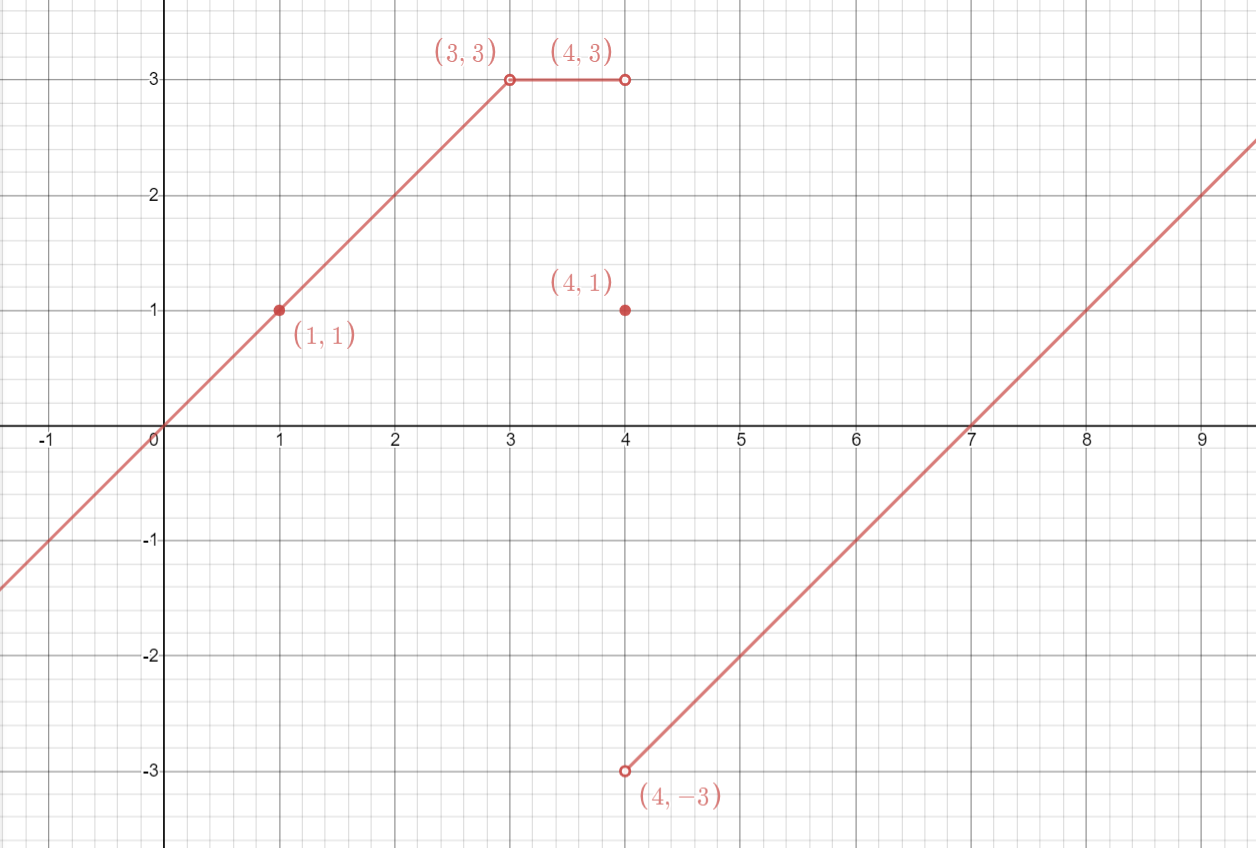
\includegraphics[width=18cm]{A1Q11.png}}
    \end{figure} 
\end{minipage}

%% I would recommend sandwiching your solution to every problem between the kind of structure I have provided below re: initial \vspace, the Solution: heading and the ending \vspace.
%\vspace{0.3cm} 
%\textbf{Solution:}\\
% Your solution starts here.
%\vspace{0.3cm}

\newpage

%% PROBLEM 12
\item Evaluate the following limits if they exist or assert that they do not exist with evidence.\\

\textbf{Solution:}
\begin{enumerate}
%a
\item[(a)] $\lim_{h\to 0}\limits \dfrac{(4+h)^2 -16}{h}$ \\
Let $L = \lim_{h\to 0}\limits \dfrac{(4+h)^2 -16}{h}$.
\begin{align}
    L &= \lim_{h\to 0}\limits \dfrac{(4+h)^2 -16}{h} \\
    L &= \lim_{h\to 0}\limits \dfrac{(4+h - 4)(4+h + 4)}{h} \\
    L &= \lim_{h\to 0}\limits \dfrac{h(8+h)}{h} \\
    L &= \lim_{h\to 0}\limits (8+h) \\
    L &= \lim_{h\to 0}\limits (8+0) \\
    L &=  8
\end{align}
\textbf{Therefore, $L = 8$.}\\
\setcounter{equation}{0}
%b
\item[(b)] $\lim_{t\to 9}\limits \dfrac{9-t}{3-\sqrt{t}}$ \\
Let $L = \lim_{t\to 9}\limits \dfrac{9-t}{3-\sqrt{t}}$
\begin{align}
    L &= \lim_{t\to 9}\limits \dfrac{9-t}{3-\sqrt{t}} \\
    L &= \lim_{t\to 9}\limits \dfrac{(3-\sqrt{t})(3+\sqrt{t})}{3-\sqrt{t}} \\
    L &= \lim_{t\to 9}\limits (3+\sqrt{t})\\
    L &= (3+\sqrt{9})\\
    L &= (3+ 3)\\
    L &= 6
\end{align}
\textbf{Therefore, $L = 6$.}\\
\setcounter{equation}{0}
\newpage
%c
\item[(c)] $\lim_{x\to -4}\limits \dfrac{\frac{1}{4}+\frac{1}{x}}{4+x}$ \\
Let $L = \lim_{x\to -4}\limits \dfrac{\frac{1}{4}+\frac{1}{x}}{4+x}$
\begin{align}
    L &= \lim_{x\to -4}\limits \left(\dfrac{1}{4}+\dfrac{1}{x}\right)\times \dfrac{1}{4+x} \\
    L &= \lim_{x\to -4}\limits \left(\dfrac{x+4}{4x}\times\dfrac{1}{x+4}\right) \\
    L &= \lim_{x\to -4}\limits \dfrac{1}{4x} \\
    L &= \dfrac{1}{-16}
\end{align}
\textbf{Therefore, $L = \dfrac{1}{-16}$}
\setcounter{equation}{0}
%d
\item[(d)] $\lim_{t\to 0}\limits \left(\dfrac{1}{t\sqrt{1+t}} - \dfrac{1}{t}\right)$ \\
Let $L = \lim_{t\to 0}\limits \left(\dfrac{1}{t\sqrt{1+t}} - \dfrac{1}{t}\right)$
\begin{align}
    L &= \lim_{t\to 0}\limits \left(\dfrac{1}{t\sqrt{1+t}} - \dfrac{1}{t}\right)\\
    L &= \lim_{t\to 0}\limits \left(\dfrac{1-\sqrt{1-t}}{t\sqrt{1+t}}\right)\\
    L &= \lim_{t\to 0}\limits \left(\dfrac{1-\sqrt{1-t}}{t\sqrt{1+t}}\times\dfrac{1+\sqrt{1+t}}{1+\sqrt{1+t}}\right)\\
    L &= \lim_{t\to 0}\limits \left(\dfrac{1-(1+t)}{t\sqrt{1+t}(1+\sqrt{1+t})}\right)\\
    L &= \lim_{t\to 0}\limits \left(\dfrac{-t}{t\sqrt{1+t}(1+\sqrt{1+t})}\right)\\
    L &= \lim_{t\to 0}\limits \left(-\dfrac{1}{\sqrt{1+t}(1+\sqrt{1+t})}\right)\\
    L &= -\dfrac{1}{2}
\end{align}
\textbf{Therefore, $L = -\dfrac{1}{2}$}
\setcounter{equation}{0}
%e
\item[(e)] $\lim_{x\to 0^-}\limits \left(\dfrac{1}{x} - \dfrac{1}{|x|}\right)$\\
Let $L = \lim_{x\to 0^-}\limits \left(\dfrac{1}{x} - \dfrac{1}{|x|}\right)$
\begin{align}
    L &= \lim_{x\to 0^-}\limits \left(\dfrac{1}{x} - \dfrac{1}{|x|}\right) \\
    L &= \lim_{x\to 0^-}\limits \left(\dfrac{1}{-0.00001} - \dfrac{1}{|-0.00001|}\right) \\
    L &= -\infty
\end{align}
Since the limit can only approach a number and $-\infty$ is not a number, the limit DNE.\\
\textbf{Therefore, $L$ does not exist.}
\end{enumerate}
\setcounter{equation}{0}
\newpage

%% PROBLEM 13
\item Prove  $\lim_{x\to 0}\limits x^4 \cos\left(\dfrac{2}{x}\right) = 0$. (Hint: Use the Squeeze Theorem) \\

\textbf{Solution:} \\
Given that the range of a cosine function is from -1 to 1, inclusive, we have the following:
    $$-1 \leq \cos\left(x\right) \leq 1$$
We know that placing a coefficient beside $x$ will not change a function's range:
    $$-1 \leq \cos\left(\dfrac{2}{x}\right) \leq 1$$
Multiply the functions by $x^4$. Note that $x^4 \geq 0$ for all real values of $x$, therefore, we do not need to change the inequality signs:
    $$-x^4 \leq x^4 \cos\left(\dfrac{2}{x}\right) \leq x^4$$
Apply the limit to each function:
    $$\lim_{x\to 0}\limits -x^4 \leq \lim_{x\to 0}\limits x^4 \cos\left(\dfrac{2}{x}\right) \leq \lim_{x\to 0}\limits x^4$$
We cannot determine the limit of $x^4 \cos\left(\dfrac{2}{x}\right)$ by substitution as it would yield an undefined value for the function in the middle (since we are dividing by zero). So, by the Squeeze Theorem, we can substitute in $x = 0$ into $-x^4$ and $x^4$ to determine $\lim_{x\to 0}\limits x^4 \cos\left(\dfrac{2}{x}\right) = 0$:
    $$-0^4 \leq \lim_{x\to 0}\limits x^4 \cos\left(\dfrac{2}{x}\right) \leq 0^4$$
    $$0 \leq \lim_{x\to 0}\limits x^4 \cos\left(\dfrac{2}{x}\right) \leq 0$$

\textbf{Therefore, by the Squeeze Theorem, $\lim_{x\to 0}\limits x^4 \cos\left(\dfrac{2}{x}\right) = 0$}
\newpage

%% PROBLEM 14
\item Show by means of an example that  $\lim_{x\to a}\limits f(x)g(x)$ might exist even though neither $\lim_{x\to a}\limits f(x)$ nor $\lim_{x\to a}\limits g(x)$ exist. \\

\textbf{Solution:} \\
Consider two functions:
$$f(x) = \sin \left(\dfrac{1}{x}\right)$$
$$g(x) = \dfrac{1}{\sin \left(\frac{1}{x}\right)}$$

We can see that $\lim_{x\to 0}\limits f(x)$ and $\lim_{x\to 0}\limits g(x)$ do not exist. To prove that $\lim_{x\to 0}\limits f(x)g(x)$ exists, let's assume that the limit does exist and that it equals $L$.
\setcounter{equation}{0}
\begin{align}
    L &= \lim_{x\to 0}\limits f(x)g(x) \\
    L &= \lim_{x\to 0}\limits \left(\sin \left(\dfrac{1}{x}\right) \dfrac{1}{\sin \left(\frac{1}{x}\right)} \right) \\
    L &= 1
\end{align}
\setcounter{equation}{0}

\textbf{Therefore, the product of two functions that do not have limits can have a limit.}

\newpage

%% PROBLEM 15
\item Determine a value for $a$ (if any) such that $\lim_{x\to -2}\limits \dfrac{3x^2 + ax + a + 3}{x^2 + x - 2}$ exists. If it exists, also determine the value of the limit. \\

\textbf{Solution:} \\
Let $f(x) = \dfrac{3x^2 + ax + a + 3}{x^2 + x - 2}$ so this function is easier to refer to in my solution.
Assume that there exists a value $a$ such that $\lim_{x\to -2}\limits f(x)$ exists and that the value of the limit equals $L$. \\

\textbf{Step 1:} Factor the denominator.
\begin{align}
    L &= \lim_{x\to -2}\limits \dfrac{3x^2 + ax + a + 3}{x^2 + x - 2} \\
    L &= \lim_{x\to -2}\limits \dfrac{3x^2 + ax + a + 3}{(x-1)(x+2)}
\end{align}
Currently, we cannot determine the limit of $f(x)$ by substitution because of the $(x+2)$ factor in the denominator. To solve this issue, we must determine a value of $a$ such that when the numerator is factored, will eliminate the $(x+2)$ in the denominator. For this to happen, $x=-2$ must be a zero of the numerator. \\

\textbf{Step 2:} Determine $a$ when $x=-2$ is a zero of the numerator of $f(x)$.\\
Let the numerator of $f(x)$ be $y$.
\begin{align}
    y &= 3x^2 + ax + a + 3 \\
    0 &= 3(-2)^2 + (-2)a + a + 3 \\
    0 &= 12 - 2a + a + 3 \\
    0 &= 15 - a \\
    a &= 15
\end{align}
\textbf{Step 3:} Sub in a = 15 into $f(x)$ to check if $\lim_{x\to -2}\limits f(x)$.
\begin{align}
    L &= \lim_{x\to -2}\limits \left(\dfrac{3x^2+15x+18}{(x-1)(x+2)} \right) \\
    L &= \lim_{x\to -2}\limits \left(\dfrac{3(x+2)(x+3)}{(x-1)(x+2)} \right) \\
    L &= \lim_{x\to -2}\limits \left(\dfrac{3(x+3)}{(x-1))} \right) \\
    L &= \lim_{x\to -2}\limits \left(\dfrac{3((-2)+3)}{((-2)-1))} \right) \\
    L &= \dfrac{3}{-3} \\
    L &= -1
\end{align}
\textbf{Therefore, there exists a value for $a$ such that $\lim_{x\to -2}\limits \dfrac{3x^2 + ax + a + 3}{x^2 + x - 2}$. That is $a = 15$ and the value of the limit is -1.}


\newpage


%% PROBLEM 16
\item Determine for which values of $x$ (if any) the function $f(x) = \begin{cases} 
      x + 2 & : x < 0 \\
      2x^2 & : 0 \le x \le 1 \\
		 2-x & : x>1 \\
   \end{cases}$ is discontinuous.\\

\textbf{Solution:} \\
Recall that all polynomial functions are continuous from $(-\infty, \infty)$. Since each of the cases in the piece-wise function $f(x)$ are polynomial functions, all of them are continuous for their respective cases. That means, the point of transition between the three cases must be discontinuous. Let's prove it. \\

If $\lim_{x\to 0}\limits (x+2) \neq \lim_{x\to 0}\limits = 2x^2$, $x=0$ is discontinuous on f(x). Likewise, if $\lim_{x\to 1}\limits 2x^2 \neq \lim_{x\to 1}\limits (2-x)$, $x=1$ is discontinuous on $f(x)$.
\setcounter{equation}{0}
\begin{align}
    &\lim_{x\to 0}\limits (x+2) = 2 \\
    &\lim_{x\to 0}\limits 2x^2 = 0
\end{align}
Since $\lim_{x\to 0}\limits (x+2) \neq \lim_{x\to 0}\limits 2x^2$, f(x) is discontinuous at $x=0$.
\begin{align}
    &\lim_{x\to 1}\limits 2x^2 = 2 \\
    &\lim_{x\to 1}\limits (2-x) = 1
\end{align}
Since $\lim_{x\to 1}\limits 2x^2 \neq \lim_{x\to 1}\limits (2-x)$, f(x) is discontinuous at $x=1$.\\

\textbf{Therefore, $f(x)$ is discontinuous at $x=0,1$.}


\newpage


%% PROBLEM 17
\item Determine the values of $a$ and $b$ such that $f(x) = \begin{cases} 
      \dfrac{x^2-4}{x-2} & : x < 2 \\
      ax^2-bx+3 & : 2 \leq x < 3 \\
		 2x-a+b & : x \ge 3 \\
   \end{cases}$ is continuous on $\mathbb{R}$.\\
\textbf{Solution:\\}
Simplify $\dfrac{x^2-4}{x-2}$.
\setcounter{equation}{0}
\begin{align}
    \dfrac{x^2-4}{x-2} &= \dfrac{(x-2)(x+2)}{x-2} \\
    &= x+2 \qquad (x \neq 2)
\end{align}
For $f(x)$ to be continuous, I must prove that each of its cases and the transition from case to case must be continuous. That means, $a$ and $b$ must result in case 1 and 2 to equalling each other $f(2)$, and case 2 and 3 to equal at $f(3)$. \\

Let's start with cases 1 and 2. Since the first case cannot be 2, we say the limit of $x+2$ as $x$ approaches 2 equals case 2. We have,
\begin{align}
    \lim_{x\to 2}\limits (x+2) &= ax^2 - bx + 3 \\
    \lim_{x\to 2}\limits ((2)+2) &= (2)^2a - (2)b + 3 \\
    4 &= 4a - 2b + 3 \\
    0 &= 4a - 2b - 1
\end{align}
Since there are two variables, $a$ and $b$, we cannot exactly solve for their values yet. Let's move on to cases 2 and 3 where they are both equal to each other at $f(3)$.
\begin{align}
    ax^2-bx+3 &= 2x-a+b \\
    (3)^2a-(3)b+3 &= 2(3)-a+b \\
    9a-3b+3 &= 6-a+b \\
    0 &= 10a -4b -3
\end{align}
Multiple both sides of line (6) by 2, we have $0 = 8a-4b-2$. Now, we can determine $a$ and $b$ by elimination.
\begin{align}
    &0 = 8a - 4b - 2 \\
    - \quad &0 = 10a -4b -3 \\
    &\rule{5cm}{0.5pt}\\
    &0 = -2a+1
\end{align}
Therefore, we have,
    $$a = \dfrac{1}{2}$$
Determine $b$ using the equation from line (11).
\begin{align}
    0 &= 4\left(\dfrac{1}{2}\right) - 2b - 1 \\
    b &= 1-2b \\
    b &= \dfrac{1}{2}
\end{align}
\textbf{Therefore, $a = \dfrac{1}{2}$, \quad $b = \dfrac{1}{2}$}.







\newpage


%% PROBLEM 18
\item Prove that there is a root of the equation $\sqrt[3]{x}=1-x$ on the interval $I=(0,1)$. (Hint: Consider the Intermediate Value Theorem) \\

\textbf{Solution:}\\
\setcounter{equation}{0}
Rearrange $\sqrt[3]{x}=1-x$.
\begin{align}
    \sqrt[3]{x} &= 1-x \\
    0 &= \sqrt[3]{x} +x - 1
\end{align}
\textit{Note:} Theorem 4.1 on page 88 states that the function $\sqrt[3]{x}$ is continuous for all $x$, when $n$ is odd. Therefore, $\sqrt[3]{x} +x - 1$ is continuous by Theorem 4.1.\\\\

Sub in $x=0, 1$ to determine the output of the endpoints on the interval $I$.
\begin{align}
    f(0) &= \sqrt[3]{0} +0 - 1 \\
    f(0) &= -1 \\
    f(1) &= \sqrt[3]{1} +1 - 1 \\
    f(1) &= 1
\end{align}
Since the endpoints yield values -1 and 1, by the IVT, $\sqrt[3]{x}=1-x$ must yield a value between -1 and 1 for $x \in I = (0,1)$. Since $-1 < 0 < 1$ and $\sqrt[3]{x}=1-x$ is continuous on the interval $I = (0,1)$, there exists a root of the equation $\sqrt[3]{x}=1-x$ on the interval $I = (0,1).$

\newpage


%% PROBLEM 19
\item Evaluate $\lim_{x\to 0}\limits \dfrac{\sqrt[3]{1+cx}-1}{x}$ where $c \in \mathbb{R^*}$. \\

\textbf{Solution:\\}
\setcounter{equation}{0}
Let $L = \lim_{x\to 0}\limits \dfrac{\sqrt[3]{1+cx}-1}{x}$.
\begin{align}
    L &= \lim_{x\to 0}\limits \dfrac{\sqrt[3]{1+cx}-1}{x} \\
    L &= \lim_{x\to 0}\limits \dfrac{(1+cx)^{\frac{1}{3}}-1^{\frac{1}{3}}}{x}
\end{align}
Let $a = 1+cx$ and $b = 1$. We have $\sqrt[3]{1+cx}-1 = a^\frac{1}{3} - b^\frac{1}{3}$. %%Recall the identity $a^3-b^3 = (a-b)(a^2+ab+b^2)$, I can see that $(a-b)$ is a factor of the identity.
\begingroup
\addtolength{\jot}{0.5em}
\begin{align}
    L &= \lim_{x\to 0}\limits \dfrac{(1+cx)^{\frac{1}{3}}-1^{\frac{1}{3}}}{x}\\
    L &= \lim_{x\to 0}\limits \dfrac{a^{\frac{1}{3}}-b^{\frac{1}{3}}}{x}\\
    L &= \lim_{x\to 0}\limits \left(\dfrac{(a^\frac{1}{3}-b^\frac{1}{3})}{x} \times \dfrac{a^{\frac{2}{3}} + a^{\frac{2}{3}}b^{\frac{2}{3}} + b^{\frac{2}{3}}}{a^{\frac{2}{3}} + a^{\frac{2}{3}}b^{\frac{2}{3}} + b^{\frac{2}{3}}}  \right) \\
    L &= \lim_{x\to 0}\limits \left(\dfrac{a-b}{x(a^\frac{2}{3} + a^\frac{2}{3}b^\frac{2}{3} + b^\frac{2}{3})}\right) \\
    L &= \lim_{x\to 0}\limits \dfrac{1+cx - 1}{2x(1+cx)^\frac{2}{3}} \\
    L &= \lim_{x\to 0}\limits \dfrac{cx}{2x(1+cx)^\frac{2}{3}} \\
    L &= \lim_{x\to 0}\limits \dfrac{c}{2(1+cx)^\frac{2}{3}} \\
    L &= \lim_{x\to 0}\limits \dfrac{c}{2(1+c(0))^\frac{2}{3}} \\
    L &= \dfrac{c}{3}
\end{align}
\endgroup

\textbf{Therefore, $L = \dfrac{c}{3}$}.

\newpage

\setcounter{equation}{0}
%% PROBLEM 20
\item Given $\lim_{x\to a}\limits (f(x)+g(x))=2$ and $\lim_{x\to a}\limits (f(x)-g(x))=1$ determine the value of $\lim_{x\to a}\limits f(x)g(x)$.\\

\textbf{Solution:\\}
Let $f(x) = m, g(x) = n$.\\
Theorem 3.1 (ii) on page 78 states that the limit of a sum equals the sum of two limits. Therefore, I can say:
\begin{align}
    2 &= \lim_{x\to a}\limits m + \lim_{x\to a}\limits n \\
    2 &= \lim_{x\to a}\limits (m + n)
\end{align}
And,
\begin{align}
    1 &= \lim_{x\to a}\limits m - \lim_{x\to a}\limits n \\
    1 &= \lim_{x\to a}\limits (m - n)
\end{align}
Let's add line (2) and (4) together.
\begin{align}
    &2 = \lim_{x\to a}\limits (m + n) \\
    + \quad &1 = \lim_{x\to a}\limits (m - n) \\
    &\rule{5cm}{0.5pt}\\
    &3 = \lim_{x\to a}\limits (m + n) + \lim_{x\to a}\limits (m - n)
\end{align}
Again, by Theorem 3.1(ii), I can rewrite line (8) as:
\begin{align}
    3 &= \lim_{x\to a}\limits (m + n) + \lim_{x\to a}\limits (m - n)\\
    3 &= \lim_{x\to a}\limits (m + n + m - n)\\
    3 &= \lim_{x\to a}\limits (2m)\\
    3 &= 2\lim_{x\to a}\limits (m) \xleftarrow[]{\text{by Theorem 3.1(i)}}\\
    \lim_{x\to a}\limits m &= \dfrac{3}{2}
\end{align}
Now that we have determined $m$, use the given equation on line (1) to determine $n$.
\begin{align}
    2 &= \lim_{x\to a}\limits m + \lim_{x\to a}\limits n \\
    2 &= \dfrac{3}{2} + \lim_{x\to a}\limits n \\
    \lim_{x\to a}\limits n &= \dfrac{1}{2}
\end{align}\\

$$\therefore \quad \lim_{x\to a}\limits f(x) = \dfrac{3}{2}\text, \qquad \lim_{x\to a}\limits g(x) = \dfrac{1}{2}$$

\newpage %newpage
Note that part (iii) of Theorem 3.1 states that the product of two limits equal the limit of the product. Therefore, I can say:
$$\lim_{x\to a}\limits f(x) \times \lim_{x\to a}\limits g(x) = \lim_{x\to a}\limits f(x)g(x)$$

Let $L = \lim_{x\to a}\limits f(x)g(x)$, we have:
\begin{align}
    L &= \lim_{x\to a}\limits f(x)g(x) \\
    L &= \lim_{x\to a}\limits \left(\dfrac{3}{2} \times \dfrac{1}{2}\right)\\
    L &= \dfrac{3}{4}
\end{align}
\textbf{Therefore, $\lim_{x\to a}\limits f(x)g(x) = \dfrac{3}{4}$}

\newpage


%% PROBLEM 21
\item The figure shows a point $P$ on the parabola $y=x^2$ and the point $Q$ where the perpendicular bisector of $OP$ intersects the y-axis. As $P$ approaches the origin along the parabola, what happens to $Q$? Does it have a limiting position? If so, determine the limiting position of $Q$.

\begin{minipage}{0.5\textwidth}
    \begin{figure}[H]
    \centering{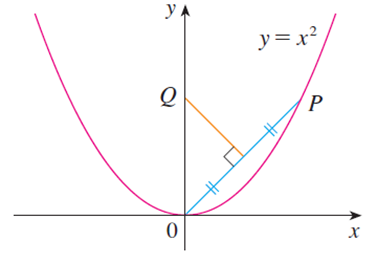
\includegraphics[width=10cm]{Q20Parabola.png}}
    \end{figure} 
\end{minipage}\\
\setcounter{equation}{0}
\textbf{Solution:\\}
\textbf{Step 1:} Find the equation of OP.\\
\textbf{Step 2:} Find the equation of the perpendicular bisector.\\
\textbf{Step 3:} Answer the question. Does it have a limiting position? if so, determine the limiting position of $Q$.\\

Let point (0,0) be $O$. \\
Let $K$ be the midpoint of $OP$. \\

First, to determine the equation of $OP$, we must determine the slope. We know that the coordinate of point $P$ be $(x,f(x))$, or, $(x, x^2)$. Since $OP$ always starts at (0,0) and the equation of $OP$ is a linear equation, we can represent it in the form $y = ax + b$. We know that $y=0$ when $x=0$, so, regardless of the value of the slope, $a$, the vertical translation, $b$, will always be 0. Therefore, the slope of $OP$ is the equation of $OP$.
\begin{align}
    m_{OP} &= \dfrac{y_2-y_1}{x_2-x_1} \\
    m_{OP} &= \dfrac{x^2-0}{x-0} \\
    m_{OP} &= \dfrac{x^2}{x} \\
    m_{OP} &= \dfrac{f(x)}{x}
\end{align}
Since $x$ is the input of the function $f(x)=x^2$, the slope is not valid, so, instead of $\dfrac{f(x)}{x}$, let the slope be $\dfrac{f(a)}{a}$ where $a$ is some constant. We now have the equation of $OP$ as $y=\dfrac{f(a)}{a}x$. However, since $OP$ starts at (0,0) and ends at point $P$, I must apply a restriction on domain to be from 0 to $a$, inclusive. Therefore, the equation of $OP$ is
    $$y = \dfrac{f(a)}{a}x \qquad (0 \leq x \leq a)$$
\newpage

Now, we need to determine the equation of $OK$. Let's start with the slope, $m_{OK}$. We know that we can determine the perpendicular bisector by taking the negative reciprocal of $m{OP}$.
\begin{align}
    m_{OK} &= -\dfrac{1}{m_{OP}} \\
    m_{OK} &= -\dfrac{a}{f(a)}
\end{align}
Now, we need to determine the vertical translation, or, the $b$ in $y=mx+b$ of $m_{OK}$. We can see that $QK$ crosses $OP$ at $\left(\dfrac{x}{2}, \dfrac{x^2}{2}\right)$, or more precisely, $\left(\dfrac{a}{2}, \dfrac{a^2}{2}\right)$. From that, we can determine $b$,
\begin{align}
    y &= ax + b \\
    \dfrac{a^2}{2} &= \left(-\dfrac{a}{f(a)}\right)\left(\dfrac{a}{2}\right) + b \\
    b &= \dfrac{a^2}{2} + \left(\dfrac{a}{f(a)}\right)\left(\dfrac{a}{2}\right)\\
    b &= \dfrac{a^2}{2} + \dfrac{a^2}{2f(a)} \\
    b &= \dfrac{a^2f(a) + a^2}{2f(a)}
\end{align}
We now have the equation of the perpendicular bisector, $OK$, as,
$$y = -\dfrac{a}{f(a)} + \dfrac{a^2f(a) + a^2}{2f(a)}$$
However, similar to the equation of $OP$, $OK$'s domain is restricted from 0 to $\dfrac{a}{2}$, inclusive. Therefore, the equation of $OK$ is,

$$y = -\dfrac{a}{f(a)} + \dfrac{a^2f(a) + a^2}{2f(a)} \qquad \left(0 \leq x \leq \dfrac{a}{2}\right)$$\\

Finally, we can now determine the limiting position of $Q$. We can see that $Q$ is located at\\

$\left(0, \dfrac{a^2f(a) + a^2}{2f(a)}\right)$. To find the limiting position of $Q$, we simply need to find $\lim_{a\to 0}\limits \left( \dfrac{a^2f(a) + a^2}{2f(a)} \right)$.\\

Let $L$ be the limiting position of $Q$. We have,
\newpage

\begin{align}
    L &= \lim_{a\to 0}\limits \left( \dfrac{a^2f(a) + a^2}{2f(a)} \right) \\
    L &= \lim_{a\to 0}\limits \left( \dfrac{a^2(a^2) + a^2}{2(a^2)} \right) \\
    L &= \lim_{a\to 0}\limits \left( \dfrac{a^4 + a^2}{2a^2} \right) \\
    L &= \lim_{a\to 0}\limits \left( \dfrac{a^2(a^2+1)}{2a^2} \right) \\
    L &= \lim_{a\to 0}\limits \left( \dfrac{a^2+1}{2} \right) \\
    L &= \lim_{a\to 0}\limits \left( \dfrac{0^2+1}{2} \right) \\
    L &= \dfrac{1}{2}
\end{align}
\textbf{Therefore, the limiting position of $Q$ d
oes exist and its coordinate is $\left(0, \dfrac{1}{2}\right)$}.





\newpage


%% PROBLEM 22
\item Prove that at any given time there are two antipodal points on the equator with the same temperature. You may assume that temperature varies continuously with position and that the equator is a circle. (Antipodal points are diametrically opposite one another).\\

\begin{minipage}{0.5\textwidth}
    Hint: We will assume that the equator is a circle and that a point on the equator can be identified by its standard position angle $\theta$. Let $T(\theta)$ represent the temperature at the point associated with the angle $\theta$ and let $H(\theta) = T(\theta) - T(\theta+\pi)$ for $\theta \in [0,\pi]$. Then $H(\theta)$ measures the difference of the temperature at pairs of diametrically opposed points. If we can show that there exists $c$ such that $H(c)=0$ then we are essentially done the proof.\\
\end{minipage}
\begin{minipage}{0.5\textwidth}
    \begin{figure}[H]
    \centering{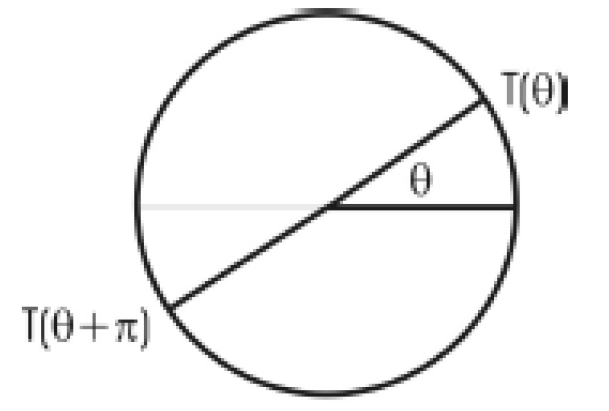
\includegraphics[width=7cm]{Q22Image.png}}
    \caption{The equator}
    \end{figure} 
\end{minipage}\\

\textbf{Solution:}\\
Let $\theta$ represent the position on the equator in radian measure.\\
Let $T(\theta)$ represent the temperature as a function of the position, $\theta$. \\
Therefore, by definition, the antipodal point of $T(\theta)$ is $T(\theta+\pi)$.\\
Let $H(\theta) = T(\theta) - T(\theta+\pi)$, or, the difference of temperature of the antipodal points.\\

We will assume that the equator is a circle which can be identified by $\theta$. Since the equator is a circle, $T(\theta)$ and $T(\theta+\pi)$ are periodic both with a period of $2\pi$. Note that $T(\theta)$ and $T(\theta+\pi)$ are continuous as temperature cannot "jump."\\

\textbf{Examining $T(\theta)$}\\
We know that $T(\theta)$ is continuous, has a period of $2\pi$, with the period $\in [0, 2\pi]$. Since $T(\theta)$ has these characteristics, it is true that $T(\theta)$ will always have an absolute minimum and an absolute maximum for $\theta \in [0, 2\pi]$ and that the absolute minimum and maximum of $T(\theta)$ for $\theta \in [0,2\pi]$ is the same as the absolute minimum and maximum of $T(\theta)$ for $\theta \in \mathbb{R}$, since $T(\theta)$ is periodic.\\

Therefore, I can say that $\exists$ $a$, $b \in [0, 2\pi]$, where $T(a)$ is the absolute minimum and $T(b)$ is the absolute maximum of $T(\theta)$.\\

\textbf{Examining $T(\theta+\pi)$}\\
We know that $T(\theta+\pi)$ is also continuous and has a period of $2\pi$, however, the period of $T(\theta+\pi) \in [\pi, 3\pi]$. This is because $T(\theta+\pi)$ is just $T(\theta)$ but translated $\pi$ units left. This means, it is also true that $T(\theta+\pi)$ will always have an absolute minimum and an absolute maximum for $\theta \in [0, 2\pi]$ and that the absolute minimum and maximum of $T(\theta+\pi)$ for $\theta \in [0,2\pi]$ is the same as the absolute minimum and maximum of $T(\theta+\pi)$ for $\theta \in \mathbb{R}$, since $T(\theta+\pi)$ is periodic.\\

Similar to $T(\theta)$, I can also say that $\exists$ $a$, $b \in [0, 2\pi]$, where $T(a+\pi)$ is the absolute minimum and $T(b+\pi)$ is the absolute maximum of $T(\theta+\pi)$.\\

\newpage

\textbf{Analysis of $T(\theta)$ and $T(\theta+\pi)$}\\
We can see that both functions are essentially the same. They have the same period in magnitude of $2\pi$, but, their periods start at different positions. In other words, $T(\theta+\pi)$ is just $T(\theta)$ but translated left by $\pi$ units. So, if we were to draw both functions, $T(\theta)$ and $T(\theta+\pi)$ on the same graph, they would be the same but staggered. This also means that both functions have the same absolute minimum and absolute maximum, just at different values of $\theta$.\\

\textbf{Examining the difference between $T(\theta)$ and $T(\theta+\pi)$ or $H(\theta)$}\\
Since $T(\theta)$ and $T(\theta+\pi)$ both have the same absolute minimum and maximum values but are placed at different positions, for all values of $\theta \in [0,2\pi]$, $H(\theta)$ will change from negative to positive and/or vice versa at least once or be equal to 0.\\

Note that the only possible case where $H(\theta)=0$ is when $T(\theta)$ and $T(\theta+\pi)$ EACH have the same absolute minimums and maximums at different positions. If so, this means that the temperature is the same everywhere on the equator, so, we are not interested in this case. Therefore, we will only focus on the other two cases where values of $H(\theta)$ changes throughout the equator.\\

Since $H(\theta)$ changes values from a negative to a positive or vice versa AT LEAST ONCE, by the IVT, $H(\theta)$ is bound to have a value of 0 at least once at $H(c)$ where $c\in[0,2\pi]$. The times $H(c) = 0$ is determined by number of times the $H(\theta)$ changes from negative to positive or vice versa.\\

Recall the definition $H(\theta) = T(\theta) - T(\theta+\pi)$. Since it is possible for $H(c) = 0$, it must be true that at any given time, $T(c) = T(c+\pi)$. If $T(c) = T(c+\pi)$ is true for any given time, it is true that at any given time, there are two antipodal points on the equator with the same temperature.


\newpage



\end{enumerate}
\end{document} 
